\documentclass{article}
\usepackage[utf8]{inputenc}
\usepackage{polski}
\usepackage[polish]{babel}
\usepackage{bbm}
\usepackage{amsmath}
\usepackage{amsthm}
\usepackage{graphicx}
\usepackage{epstopdf}
\usepackage{float}
\usepackage{hyperref}
\usepackage{cleveref}

\newtheorem{defi}{Definicja}
\newtheorem{twr}{Twierdzenie}
\newtheorem*{dd}{Dowód}

\crefname{twr}{Twierdzenie}{Twierdzenia}

\DeclareMathOperator{\sign}{sign}
\DeclareMathOperator{\arctg}{arctg}

\newcommand{\twopartdef}[4]
{
	\left\{
		\begin{array}{ll}
			#1 & \mbox{dla } #2 \\
			#3 & \mbox{dla } #4
		\end{array}
	\right.
}


\author{Jarosław Dzikowski 273233}
\date{Wrocław, \today}
\title{\textbf{Pracownia z analizy numerycznej} \\ Sprawozdanie do zadania \textbf{P.3.11}}
\begin{document}
\maketitle
\section{Uwagi techniczne}
Program można uruchomić normalnie z wiersza poleceń. Wypisze on wartości całek, przybliżenia całek wyliczone
przez metodę Romberga kończoną warunkiem podanym w treści zadania, oraz wartości wyliczone przez
metodę Romberga wyliczającą $K$ poziomów tablicy Romberga.
\newline
\newline
Oprócz tego program wypisze pełne tablice błędów dla pięciu badanych funkcji. Dla pierwszych trzech tablica będzie
wymiaru 10x10, natomiast dla ostatnich dwóch tablica będzie miała rozmiar 20x20, co może być kłopotliwe
do przeglądania.
\newline
\newline
Sprawozdanie należy kompilować z wiersza poleceń będąc wewnątrz katalogu doc.
Do skompilowania sprawozdania wymagana jest obecność folderu ,,wykresy'' z wykresami w formacie eps, które następnie będą zamieszczone w sprawozdaniu. Folder ,,wykresy'' znajduje się w folderze ,,doc''.

\section{Wstęp}
W tym zadaniu zbadamy metodę Romberga całkowania numerycznego. Zbadamy jej zachowanie oraz porównamy jej rezultaty z innymi metodami.


\section{Wprowadzenie}
Zagadnienie całkowania nie jest nikomu obce. Często chcielibyśmy policzyć wartość jakiejś całki, lecz nie zawsze jest to takie proste.
Funkcja może być zbyt trudna do scałkowania lub możemy chcieć scałkować wiele funkcji, których wzorów oraz przedziałów całkowania nie znamy zawczasu.
Wtedy musimy skorzystać z jakiejś uniwersalnej metody obliczania przybliżonej wartości całki. Jedną z takich metod jest metoda Romberga.

\subsection{Kwadratury liniowe}
Zacznijmy od wprowadzenia pojęcia kwadratury. Niech $\mathbbm{F} = \mathbbm{F}[a,b]$ będzie zbiorem funkcji całkowalnych w przedziale [a,b].
Jeśli $f$ jest ciągła w [a,b), to $f \in \mathbbm{F}$. \\
Jeśli $f$ jest funkcją ograniczoną i ma skończenie wiele punktów nieciągłości w [a,b], to $f \in \mathbbm{F}$.
Całka $I: \mathbbm{F} \to \mathbbm{R}$ zapisuje się następująco
\begin{equation*}
	I(f) = \int_a^b f(x) dx
\end{equation*}
W przypadku całki z daną funkcją wagową $p$ mamy
\begin{equation*}
	I_p(f) = \int_a^b p(x) f(x) dx
\end{equation*}
Oczywiście, z własności całki wiemy, że $I$ spełnia następujące właśności:
\begin{equation*}
	(1) \ I(f + g) = \int_a^b (f+g)(x) dx = \int_a^b f(x) + g(x) dx = \int_a^b f(x) dx \ + \int_a^b g(x) dx = I(f) + I(g)
\end{equation*}
\begin{equation*}
	(2) \ I(\alpha f) = \int_a^b \alpha f(x) dx = \alpha \int_a^b f(x) dx = \alpha I(f)
\end{equation*}
\begin{equation*}
	(3) \ I(0) = \int_a^b 0 \ dx = 0
\end{equation*}
Zatem $I: \mathbbm{F} \to \mathbbm{R}$ jest \emph{funkcjonałem liniowym}.
\begin{defi}[Kwadratura liniowa]
	Funkcjonał $Q_n: \mathbbm{F} \to \mathbbm{R}$ postaci
	\begin{equation}
		Q_n(f) = \sum_{k = 0}^n A_k f(x_k),
	\end{equation}
	gdzie $A_k \in \mathbbm{R}$, oraz $x_0, x_1, ..., x_n \in [a,b]$ są parami różnymi punktami,
	nazywamy kwadraturą liniową. $A_k$ nazywamy współczynnikami kwadratury, natomiast $x_k$ węzłami kwadratury.
\end{defi}
Kwadratura jest zdefiniowana za pomocą $A_k$ i $x_k$. Każda kwadratura $Q_n$ jest w pewnym stopniu oddalona od całki.
\begin{defi}[Reszta kwadratury]
	Resztą kwadratury $Q_n$ nazywamy
	\begin{equation}
		R_n(f) = I(f) - Q_n(f)
	\end{equation}
\end{defi}
Niektóre kwadratury potrafią dawać dokładne wyniki całkowania dla wielomianów pewnego stopnia.
Dlatego wprowadzono pojęcie rzędu kwadratury.
\begin{defi}[Rząd kwadratury]
	Powiemy, że $Q_n$ jest rzędu $r$, jeśli
	\begin{equation*}
		i) \ \forall_{q \in \Pi_{r-1}} Q_n(q) = I(q)
	\end{equation*}
	\begin{equation*}
		ii) \ \exists_{q \in \Pi_r} Q_n(q) \neq I(q)
	\end{equation*}
\end{defi}
Każda kwadratura ma swoje limity i nie potrafi dokładnie scałkować każdego wielomianu.
\begin{twr}[Maksymalny rząd kwadratury]
	Rząd kwadratury $Q_n$ nie przekracza $2n + 2$.
\end{twr}
\begin{dd}
	\normalfont
	Niech $w(x) = [(x - x_0)(x - x_1) ... (x - x_n)]^2 \in \Pi_{2n + 2}$. Mamy
	\begin{equation*}
		Q_n(w) = \sum_{k = 0}^n A_k w(x_k) = 0 \neq I(w) = \int_a^b w(x) dx > 0
	\end{equation*}
	Podaliśmy przykład wielomianu stopnia $2n + 2$, dla którego kwadratura $Q_n$ nie osiąga dokładnej wartości całki.
	\qed
\end{dd}


\subsection{Kwadratury interpolacyjne}
Jak już wiemy, kwadratury zależą od doboru współczynników ${A_k}$ oraz węzłów ${x_k}$ kwadratury.
Co gdyby zamiast całkować funkcję $f$ spróbować scałkować wielomian interpolujący tę funkcję?
Ponieważ wielomian interpolujący jest swego rodzaju przybliżeniem $f$, liczymy na to, że całka z tego wielomianu będzie bliska całce z funkcji $f$.
\begin{defi}[Kwadratura interpolacyjna]
	Kwadraturą interpolacyjną nazwiemy kwadraturę $Q_n$, taką że
	\begin{equation*}
		Q_n(f) = I(L_n),
	\end{equation*}
	gdzie $L_n$ jest wielomianem interpolacyjnym stopnia $\leq n$ dla funkcji $f$.
\end{defi}
Wiemy, czym jest kwadratura interpolacyjna. Niestety dalej nie znamy jej współczynników ani węzłów.

\begin{twr}[Współczynniki oraz węzły kwadratury interpolacyjnej]
	Niech $L_n$ będzie n-tym wielomianem interpolacyjnym dla funkcji $f$ wyrażającym się wzorem
	\begin{equation*}
		L_n = \sum_{k = 0}^n f(x_k) \lambda_k
	\end{equation*}
	Wtedy $Q_n$ wyraża się wzorem
	\begin{equation*}
		Q_n = \sum_{k = 0}^n A_k f(x_k)
	\end{equation*}
	gdzie
	\begin{equation*}
		A_k = \int_a^b \lambda_k(x) dx = \int_a^b \left ( \prod_{\substack{j = 0 \\ j \neq k}}^n \frac{(x - x_j)}{(x_k - x_j)} \right ) dx
	\end{equation*}
	a $x_k$ są węzłami interpolacji wielomianu $L_n$.
\end{twr}
\begin{dd}
	\normalfont
	Ponieważ $Q_n(f) = I(L_n)$, wiemy, że $Q_n(L_n) = I(L_n)$, więc
	\begin{equation*}
		Q_n(L_n) = I(L_n) = \int_a^b  \sum_{k = 0}^n f(x_k) \lambda_k(x)  dx =
	\end{equation*}
	\begin{equation*}
		= \sum_{k = 0}^n f(x_k) \int_a^b \lambda_k(x) dx
	\end{equation*}
	\qed
\end{dd}

\begin{twr}[]
	$Q_n$ jest kwadraturą interpolacyjną wtedy i tylko wtedy, gdy rząd $Q_n$ jest równy co najmniej $n + 1$.
\end{twr}
\begin{dd}
	\normalfont
	$\implies$ :\\
	$Q_n(f) = I(L_n[f])$. Jeśli $f \in \Pi_n$, to $f = L_n[f]$. Stąd mamy rząd przynajmniej n + 1. \\
	$\impliedby$ :\\
	Niech $A_k$ będą współczynnikami $Q_n$, a $x_k$ węzłami $Q_n$ i $Q_n$ ma rząd $r \geq n + 1$. Zdefiniujemy $\lambda_k$ w sposób następujący
	\begin{equation*}
		\lambda_k = \prod_{\substack{j = 0 \\ j \neq k}}^n \frac{(x - x_j)}{(x_k - x_j)} \in \Pi_n
	\end{equation*}
	Zatem $Q_n(\lambda_k) = I(\lambda_k)$.
	Weźmy dowolne $f$. $L_n = \sum_{k = 0}^n f(x_k) \lambda_k$ interpoluje $f$ w węzłach kwadratury.
	$Q_n(f) = \sum_{k = 0}^n A_k f(x_k)$. Całka z $\lambda_k$ okazuje się być równa k-temu współczynnikowi kwadratury $Q_n$.
	\begin{equation*}
		I(\lambda_k) = Q_n(\lambda_k) = \sum_{j = 0}^n A_j \lambda_k(x_j) = A_k
	\end{equation*}
	Znając $A_k$ możemy wstawić je do wzoru na $Q_n(f)$.
	\begin{equation*}
		Q_n(f) = \sum_{k = 0}^n A_k f(x_k) = \sum_{k = 0}^n I_n(\lambda_k) f(x_k) = I(L_n[f])
	\end{equation*}
	Skoro $Q_n(f) = I(L_n[f])$, to $Q_n$ jest kwadraturą interpolacyjną.
	\qed
\end{dd}

\subsection{Kwadratury Newtona-Cotesa}
Kwadratury interpolacyjne, tak samo jak wielomiany interpolacyjne, zależą od doboru węzłów interpolacji.
Kwadratury Newtona-Cotesa używają najprostszych węzłów - węzłów równoodległych.
\begin{defi}[Kwadratura Newtona-Cotesa]
	Kwadraturą Newtona-Cotesa nazywamy kwadraturę interpolacyjną o węzłach równoodległych.
	\begin{equation*}
		Q_n^{NC}(f) = \sum_{k = 0}^n A_k f(x_k)
	\end{equation*}
	gdzie $x_k = a + k h, h = \frac{b - a}{n}$, $A_k = \int_a^b \lambda_k(x) dx$.
\end{defi}
Okazuje się, że dla kwadratur Newtona-Cotesa, współczynniki $A_k$ da się zapisać nieco inaczej
\begin{twr}[Współczynniki kwadratury Newtona-Cotesa]
	Niech $h = \frac{b - a}{n}$ będzie odległością między sąsiednimi węzłami.
	Wtedy współczynniki $A_k$ kwadratury Newtona-Cotesa $Q_n^{NC}$ wyrażają się wzorem
	\begin{equation*}
		A_k = h \cdot (-1)^{n - k} \cdot \frac{1}{k! (n-k)!} \cdot \int_a^b \left ( \prod_{\substack{j = 0 \\ j \neq k}}^n \frac{(x - x_j)}{(x_k - x_j)}\right ) dt
	\end{equation*}
\end{twr}

Dowodzi się, że błąd kwadratur Newtona-Cotesa wyraża się następująco
\begin{equation*}
	R_n(f) = \twopartdef {\frac{f^{(n + 1)}(\xi)}{(n+1)!} \int_a^b p_{n + 1}(x) dx} {2\not| n} {\frac{f^{(n + 2)}(\eta)}{(n+1)!} \int_a^b x \ p_{n + 1}(x) dx} {2 | n}
\end{equation*}
gdzie $p_{n+1}(x) = (x - x_0) (x - x_1) ... (x - x_n)$. \\
\textbf{Wniosek: }Kwadratura Newtona-Cotesa $Q_n^{NC}$ jest rzędu $\twopartdef {n + 1} {2\not| n} {n + 2} {2 | n}$.

Najbardziej znaną kwadraturą Newtona-Cotesa jest ta dla $n = 1$. $Q_1^{NC}$ z węzłami $x_0 = a, x_1 = b$, $h = b - a$ nazywamy \emph{wzorem trapezów}.
Mamy $A_0 = A_1 = \frac{h}{2}$.
\begin{equation}
	T(f) = Q_1^{NC}(f) = \frac{b - a}{2} [f(a) + f(b)]
\end{equation}
Za pomocą wzoru trapezów jesteśmy w stanie poprawnie scałkować każdą funkcję stałą oraz liniową.
Błąd wzoru trapezów $R_1(f)$ jest równy
\begin{equation*}
	R_1(f) = \frac{f''(\xi)}{2} \int_a^b (x - a)(x - b) dx = - \frac{(b - a)^3}{12} f''(\xi)
\end{equation*}

Dla $n = 2$ otrzymujemy \emph{wzór Simpsona}:
\begin{equation*}
	h = \frac{b - a}{2}, \ x_0 = a, \ x_1 = \frac{a + b}{2}, \ x_2 = b,
\end{equation*}
\begin{equation*}
	A_0 = A_2 = \frac{h}{3}, \ A_1 = 4 \frac{h}{3}
\end{equation*}
\begin{equation}
	S(f) = Q_2^{NC}(f) = \frac{b - a}{6}[f(a) + 4f\left(\frac{a + b}{2}\right) + f(b)]
\end{equation}
Rząd wzoru Simpsona wynosi 4, więc możemy poprawnie scałkować nawet wielomian trzeciego stopnia.
Błąd wzoru Simpsona wynosi
\begin{equation*}
	R_2(f) = \frac{f^{(4)}(\eta)}{4!} \int_a^b x \cdot \left(x - a\right)\left(x - \frac{a+b}{2}\right)\left(x - b\right) dx =
\end{equation*}
\begin{equation*}
	= - \frac{1}{90} \left(\frac{b - a}{2} \right)^5 f^{(4)}(\eta) = - \frac{h^5}{90} f^{(4)}(\eta)
\end{equation*}

Wykazuje się, że istnieją takie funkcje ciągłe, dla których ciąg kwadratur Newtona-Cotesa nie jest
zbieżny do całki $\int_b^a f$. Między innymi z tego powodu nie stosuje się w praktyce kwadratur Newtona-Cotesa wyższych
rzędów. Na ogół bardziej celowy jest podział przedziału całkowania $[a, b]$ na $n$ równych podprzedziałów
$[t_k, t_{k+1}]$, wyznaczony przez punkty $t_k = a + kh (k = 0, 1, \ldots , n)$, gdzie $h = \frac{b - a}{n}$, a następnie
zastosowanie w każdym z nich kwadratury Newtona-Cotesa niskiego rzędu. Otrzymujemy w ten sposób
\emph{kwadratury złożone} Newtona-Cotesa, służące do obliczania całki w całym przedziale $[a, b]$.
\newline
\newline
Jeśli w każdym z podprzedziałów $[t_k, t_{k+1}]$ użyć wzoru trapezów
\begin{equation*}
	\int_{t_k}^{t_{k + 1}} f(x) dx = \frac{h}{2}[f(t_k) + f(t_{k + 1})] - \frac{h^3}{12} f^{\prime\prime}(\xi_k),
\end{equation*}
gdzie $\xi_k \in (t_k,t_{k + 1})$, to otrzymamy
\begin{equation*}
	\int_a^b f(x) dx = \sum_{k = 0}^{n - 1} \int_{t_k}^{t_{k + 1}} f(x) dx = T_n(f) + R_n^T(f),
\end{equation*}
gdzie $T_n$ jest kwadraturą nazywaną \emph{złożonym wzorem trapezów}, określoną wzorem
\begin{equation*}
	T_n(f) = h {\sum_{k = 0}^n} {}^{\prime\prime} f(t_k),
\end{equation*}
gdzie $\sum {}^{\prime}$ oznacza sumę z pierwszym składnikiem podzielonym przez dwa, a $
sum {}^{\prime\prime}$ oznacza sumę z pierwszym i ostatnim składnikiem podzielonym przez dwa.
\newline
\newline
$R_n^T$ jest resztą tej kwadratury, równą
\begin{equation*}
	R_n^T(f) = -\frac{h^3}{12} \sum_{k = 0}^{n - 1} f^{\prime\prime}(\xi_k) = - n \frac{h^3}{12} f^{\prime\prime} (\xi) = -(b - a)\frac{h^2}{12} f^{\prime\prime} (\xi)
\end{equation*}
dla pewnego $\xi \in (a,b)$, pod warunkiem, że $f \in C^2[a,b]$.\\
Pokażemy, że złożony wzór trapezów przy $n \to \infty$ zbiega do wartości całki.
\begin{twr}[Zbieżność złożonego wzoru trapezów]
	\label{twr5}
	Niech $T_n(f)$ będzie wartością złożonego wzorów trapezów dla funkcji $f$ w przedziale całkowania $[a,b]$.
	Wtedy zachodzi
	\begin{equation*}
		\lim_{n \to \infty} T_n(f) = \int_a^b f(x) dx
	\end{equation*}
\end{twr}
\begin{dd}
	\normalfont
	Niech $s_n$ będzie dolną sumą częściową całkowania, a $S_n$ będzie górną sumą częściową całkowania. Przedział całkowania dzielimy na $n$ przedziałów długości
	$\frac{b - a}{n}$.
	\begin{equation*}
		s_n = \sum_{i = 0}^{n - 1} h \cdot \min_{x \in [a + ih, a + (i+1)h]} f(x) \quad S_n = \sum_{i = 0}^{n - 1} h \cdot \max_{x \in [a + ih, a + (i + 1)h]} f(x)
	\end{equation*}
	Oczywiście złożony wzór trapezów $T_n(f)$ wynosi
	\begin{equation*}
		T_n(f) = \sum_{i = 0}^{n - 1} h \left( \frac{f(a + ih) + f(a + (i + 1)h)}{2}\right)
	\end{equation*}
	Zatem możemy oszacować $T_n(f)$ używając sum częściowych
	\begin{equation*}
		\sum_{i = 0}^{n - 1} h \cdot \min_{x \in [a + ih, a + (i+1)h]} f(x) \leq \sum_{i = 0}^{n - 1} h \left( \frac{f(a + ih) + f(a + (i + 1)h)}{2}\right) \leq \sum_{i = 0}^{n - 1} h \cdot \max_{x \in [a + ih, a + (i + 1)h]} f(x)
	\end{equation*}
	Następnie ponieważ $\lim_{n \to \infty} s_n = \int_a^b f(x) dx = \lim_{n \to \infty} S_n$, to z reguły trzech ciągów otrzymujemy
	$\lim_{n \to \infty} T_n(f) = \int_a^b f(x) dx$.
	\qed
\end{dd}
Niech n będzie liczbą parzystą, $n = 2m$. Załóżmy, że $f \in C^4[a,b]$ i podzielmy przedział całkowania
na $m$ podprzedziałów $[t_k, t_{k + 1}]$ o długości $2h$, a następnie zastosujmy do całki w każdym
podpzedziale wzór Simpsona
\begin{equation*}
	\int_{t_{2k}}^{t_{2k + 2}} f(x) dx = \frac{2h}{6}[f(t_{2k}) + 4 f(t_{2k + 1}) + f(t_{2k + 2})] - \frac{h^5}{90} f^{(4)} (\eta_k),
\end{equation*}
gdzie $\eta_k \in (t_{2k}, t_{2k + 2})$. W efekcie otrzymujemy
\begin{equation*}
	\int_a^b f(x) dx = \sum_{k = 0}^{m - 1} \int_{t_{2k}}^{t_{2k + 2}} f(x) dx = S_n(f) + R_n^S(f),
\end{equation*}
gdzie $S_n(f)$ jest \emph{złożonym wzorem Simpsona}:
\begin{equation*}
	S_n(f) = \frac{h}{3}[f(t_0)\ + 4 f(t_1)\ + 2f(t_2)\ + 4f(t_3)\ + 2f(t_4)\ + \ldots\ + 2f(t_{2m - 2})\ + 4f(t_{2m - 1})\ + f(t_{2m})] =
\end{equation*}
\begin{equation*}
	= \frac{h}{3}[2 \sum_{k = 0}^m {}^{\prime\prime} f(t_{2k}) + 4 \sum_{k = 1}^m f(t_{2k - 1})],
\end{equation*}
a $R_n^S(f)$ jest resztą tego wzoru
\begin{equation*}
	R_n^S(f) = - \frac{h^5}{90} \sum_{k = 0}^{m - 1} f^{(4)}(\eta_k) = - m \frac{h^5}{90} f(\eta) = -(b - a) \frac{h^4}{180} f^{(4)} (\eta),
\end{equation*}
gdzie $\eta \in (a,b)$.
\newline
\newline
Ze wzorów na reszty złożonych wzorów trapezów i Simpsona wynika, że dla dostatecznie regularnych funkcji $f$ całka $I(f)$ może być przybliżona
dowolnie blisko za pomocą $T_n(f)$ lub $S_n(f)$, pod warunkiem, że weźmiemy dostatecznie małe $h$. Zachodzi zatem
\begin{equation*}
	\lim_{n \to \infty} T_n(f) = \lim_{n \to \infty} S_n(f) = I(f)
\end{equation*}
Dowód jest analogiczny do dowodu ~\cref{twr5}: ograniczamy złożoną kwadraturę przez sumy częściowe dolne i górne całkowania.
\newline
\newline
Problemem dla kwadratur Newtona-Cotesa są funkcje, dla których przedział całkowania nie zawiera się w dziedzinie funkcji.
Przykładem jest następująca całka $\int_{-1}^1 \frac{1}{\sqrt{1 - x^2}} dx$ Ponieważ w punktach $x = -1$ oraz $x = 1$ funkcja jest nieokreślona,
nie możemy zastosować kwadratur Newtona-Cotesa.

\section{Metoda Romberga}
W tej sekcji posłużymy się poznanymi już złożonymi kwadraturami Newtona-Cotesa do wyprowadzenia metody Romberga
całkowania numerycznego.
\subsection{Twierdzenie Eulera - Maclaurina}
Oznaczmy przez $B_k$ k-tą liczbę Bernouliego. Przypomnijmy:
\begin{equation*}
	\frac{x}{e^x - 1} = \sum_{n = 0}^\infty \frac{B_n}{n!} x^n
\end{equation*}

\begin{defi}[Twierdzenie Eulera - Maclaurina]
	Niech $f \in C^{2m + 2}[a,b]$. Wtedy reszta złożonego wzoru trapezów wyraża się wzorem
	\begin{equation}
		R_n^T(f) = \frac{c_1}{n^2} + \frac{c_2}{n^4} + \frac{c_3}{n^6} + \ldots + \frac{c_m}{n^{2m}} + \frac{d(n)}{n^{2m + 2}} \; (n \to \infty),
	\end{equation}
	gdzie $d(n)$ jest funkcją ograniczoną, tzn. $\exists_{M} \forall_{n} |d(n)| < M$ oraz
	\begin{equation*}
		c_k = \frac{(b - a)^{2k}}{(2k)!} B_{2k} [f^{(2k - 1)}(b) - f^{(2k - 1)}(a)]
	\end{equation*}
\end{defi}

Sprawdźmy na jakimś przykładzie, jak bardzo potrafimy przyspieszyć zbieżność metody trapezów. Niech $f(x) = \frac{1}{x},\ a = 1,\ b = 3$.
\begin{equation*}
	I(f) = \int_a^b \frac{1}{x} dx = \ln 3 \approx 1.098612
\end{equation*}
Teraz policzmy tę samą całkę złożoną metodą trapezów dzieląc przedział całkowania na 64 podprzedziały.
Wydawałoby się intuicyjne, że jeśli podzielimy przedział całkowania na dwa razy więcej przedziałów,
to uzyskamy dużo lepszy wynik. Niestety okazuje się, że tak nie jest.
\begin{equation*}
	T_{64} = \textbf{1.0986}85 \quad T_{128} = \textbf{1.0986}30
\end{equation*}
Złożona metoda trapezów dla podwojonej liczby przedziałów nie dała większej liczby cyfr dokładnych.
Spójrzmy na błąd złożonej metody trapezów przy podziale na $n$ przedziałów
\begin{equation*}
	R_n^T(f) = \frac{c_1}{n^2} + \frac{c_2}{n^4} + \ldots + \frac{d(n)}{n^{2m + 2}} \quad\quad R_n^T = I - T_n
\end{equation*}
A następnie na błąd przy podziale na $2n$ przedziałów
\begin{equation*}
	R_{2n}^T(f) = \frac{c_1}{4n^2} + \frac{c_2}{16n^4} + \ldots  \quad\quad R_{2n}^T = I - T_{2n}
\end{equation*}
Spróbujmy usunać $\frac{c_1}{n^2}$ - najbardziej znaczący ze składników reszty $R_n^T(f)$
\begin{equation*}
	4R_{2n}^T(f) - R_n^T(f) = -\frac{3}{4} c_2 \frac{1}{n^4} - \frac{15}{16} c_3 \frac{1}{n^{16}} - \ldots \quad\quad 4R_{2n}^T - R_n^T = 3I - (4T_{2n} - T_n)
\end{equation*}
Zatem dla
\begin{equation*}
	T_n^\prime = \frac{4T_{2n} - T_n}{3}
\end{equation*}
zachodzi
\begin{equation*}
	R_n^\prime = I - T_n^\prime = - \frac{c_2}{4n^4} - \frac{5}{16n^6} + \ldots
\end{equation*}
Sprawdźmy teraz, jaki efekt otrzymamy w porównaniu do wcześniej wyliczonych $T_{64}$ i $T_{128}$.
\begin{equation*}
	T_{64}^\prime = \frac{4T_{128} - T_{64}}{3} = \textbf{1.098612}...
\end{equation*}
Widać, że zwiększyliśmy liczbę cyfr dokładnych.

\subsection{Tablica Romberga}
Skoro udało nam się wyeliminować najbardziej znaczący składnik błędu złożonego wzoru
trapezów $R_n^T$, to dlaczego mielibyśmy zatrzymać się w tym miejscu? W analogiczny sposób jak poprzednio możemy usunąć
kolejny najbardziej znaczący składnik reszty: $\frac{1}{n^4}$. Następnie możemy usuwać kolejne najbardziej znaczące
składniki. W ten właśnie sposób działa metoda Romberga.
\newline
\newline
W metodzie tej skonstruujemy trójkątną tablicę kolejnych ,,przyspieszeń'' złożonego wzoru trapezów.
Niech
\begin{equation*}
T_{0,k} = T_{2^k}
\end{equation*}
Pierwsza kolumna tablicy wypełniona jest złożonymi wzorami trapezów dla podziału
przedziału całkowania na $2^k$ równych części. Niech $h_k = \frac{b - a}{2^k}$ oznacza długośc podprzedziału.
\newline
\newline
Kolejne kolumny tablicy konstruujemy poznaną przez nas metodą:
\begin{equation}
	T_{m,k} = \frac{4^m T_{m - 1, k + 1} - T_{m - 1, k}}{4^m - 1}
\end{equation}
W efekcie otrzymujemy następującą tablicę:

\begin{table}[h]
\centering
\begin{tabular}[c]{|c c c c c c|}
\hline
$T_{0,0}$ &  &  &  &  & \\
$T_{0,1}$ & $T_{1,0}$ &  &  & & \\
$T_{0,2}$ & $T_{1,1}$ & $T_{2,0}$ & & & \\
$T_{0,3}$ & $T_{1,2}$ & $T_{2,1}$ & $T_{3,0}$ &  &  \\
\dots & \dots & \dots & \dots & \dots & \\
$T_{0,k}$ & $T_{1,k - 1}$ & $T_{2,k - 2}$ & $T_{3,k - 3}$ & \dots & $T_{k,0}$ \\
\hline
\end{tabular}
\caption{Tablica Romberga.}
\end{table}

\begin{twr}[Druga kolumna tablicy Romberga]
	W drugiej kolumnie tablicy Romberga znajdują się złożone wzory Simpsona dla $n = 2^i, (i = 0, 1, \ldots)$, tj.
	\begin{equation*}
		T_{1, k} = S_{2^{k+1}}
	\end{equation*}
\end{twr}
\begin{dd}
	\normalfont
	Niech $n = 2m$. Rozwińmy wzór na $S_n$.
	\begin{equation*}
		S_n(f) = \frac{h}{3}[f(t_0)\ + 4 f(t_1)\ + 2f(t_2)\ + 4f(t_3)\ + 2f(t_4)\ + \ldots\ + 2f(t_{2m - 2})\ + 4f(t_{2m - 1})\ + f(t_{2m})] =
	\end{equation*}
	\begin{equation*}
		= \frac{h}{3}[2 \sum_{k = 0}^m {}^{\prime\prime} f(t_{2k}) + 4 \sum_{k = 1}^m f(t_{2k - 1})] =
	\end{equation*}
	\begin{equation*}
		= \frac{h}{3}[4 \sum_{k = 0}^m {}^{\prime\prime} f(t_{2k}) + 4 \sum_{k = 1}^m f(t_{2k - 1})] - \frac{h}{3} 2 \sum_{k = 0}^m {}^{\prime\prime} f(t_{2k}) =
	\end{equation*}
	\begin{equation*}
		= \frac{4 T_n(f) - T_m(f)}{3}
	\end{equation*}
	Widzimy, że otrzymany wzór jest taki sam jak wzór na drugą kolumnę w tablicy Romberga. Stąd
	\begin{equation*}
		S_{2^{k+1}} = \frac{4T_{2^{k+1}} - T_{2^k}}{3} = \frac{4T_{0,k+1} - T_{0,k}}{3} = T_{1,k}
	\end{equation*}
	\qed
\end{dd}

\begin{twr}[Zbieżność metody Romberga]
	Niech $T_{i,j}$ będą wyrazami tablicy Romberga. Wtedy zachodzi
	\begin{equation*}
		\lim_{m \to \infty} T_{m, 0} = \int_a^b f(x) dx
	\end{equation*}
\end{twr}
\begin{dd}
	\normalfont
	Dowód analogiczny do dowodu ~\cref{twr5}. Zawsze możemy ograniczyć $T_{i,j}$ przez sumy częściowe całkowania dolną oraz górną.
	Następnie z twierdzenia o trzech ciągach pokazujemy, że $\lim_{n \to \infty} T_{n,0} = \int_a^b f(x) dx$.

	Ograniczenie przez sumy częściowe całkowania można udowodnić indukcyjnie
	\begin{enumerate}
		\item $m = 0$
			\newline
			Dla $m = 0$ mamy do czynienia ze złożonym wzorem trapezów. Zbieżność ta została udowodniona wcześniej.
		\item Załóżmy indukcyjnie, że dla $m \geq 0$ teza zachodziła, tj.
			\begin{equation*}
				s_{m,k} \leq T_{m,k} \leq S_{m,k} ,
			\end{equation*}
			gdzie $s_{m,k}$ oraz $S_{m,k}$ są odpowiednio dolną oraz górną sumą częściową całkowania.
			Pokażemy, że dla $m + 1$ $T_{m + 1,k}$ też da się ograniczyć przez sumy częściowe.
			Z rekurencyjnej zależności wzoru Romberga mamy
			\begin{equation*}
				T_{m+1,k} = \frac{4^{m + 1} T_{m,k + 1} - T_{m, k}}{4^{m + 1} - 1}
			\end{equation*}
			Na mocy założenia indukcyjnego zachodzą dwie nierówności
			\begin{equation*}
				s_{m,k + 1} \leq T_{m,k + 1} \leq S_{m,k + 1} \quad\quad s_{m,k} \leq T_{m,k} \leq S_{m,k}
			\end{equation*}
			Zatem zachodzi następująca nierówność
			\begin{equation*}
				4^{m+1} s_{m,k+1} - s_{m,k} \leq 4^{m+1} T_{m,k+1} - T_{m,k} \leq 4^{m+1} S_{m,k+1} - S_{m,k}
			\end{equation*}
			Poneważ $s_{m,k} \leq s_{m,k+1}$ oraz $S_{m,k+1} \leq S_{m,k}$ mamy
			\begin{equation*}
				(4^{m+1} - 1) s_{m,k} \leq 4^{m+1} T_{m,k+1} - T_{m,k} \leq (4^{m+1} - 1) S_{m,k}
			\end{equation*}
			Dzieląc obustronnie przez $(4^{m+1} - 1)$ otrzymujemy
			\begin{equation*}
				s_{m,k} \leq \frac{4^{m+1} T_{m,k+1} - T_{m,k}}{4^{m+1} - 1} \leq S_{m,k}
			\end{equation*}
			Otrzymujemy zatem tezę
			\begin{equation*}
				s_{m+1,k} = s_{m,k} \leq T_{m+1,k} \leq S_{m,k} = S_{m+1,k}
			\end{equation*}
			\qed
	\end{enumerate}
\end{dd}

Przy obliczaniu pierwszej kolumy, czyli złożonych wzorów trapezów dla $n = 2^i$ możemy wykonać małą optymalizację,
która pozwoli nam policzyć wszystkie $T_{0,0}, T_{0,1}, \ldots, T_{0,k}$ czyli de facto $T_1, T_{2}, \ldots, T_{2^k}$
dodając wartość funkcji całkowanej w każdym z $2^k$ węzłów tylko jeden raz. Niech $h_i = \frac{b-a}{2^i}$.
\begin{equation*}
	T_{2^{i+1}} = \frac{1}{2} T_{2^i} + \frac{h_i}{2} \sum_{k = 1}^{2^i} f\left(a + k h_i - \frac{h_i}{2}\right)
\end{equation*}
W załączonym programie pierwsza kolumna tablicy Romberga obliczana jest właśnie w taki sposób.\\
Należy wspomnieć, że ponieważ w metodzie Romberga wykorzystujemy kwadratury dla węzłów równoodległych, nie możemy
scałkować funkcji, dla których przedział całkowania nie zawiera się w ich dziedzinach.

\section{Doświadczenia}
Przejdźmy teraz do prezentacji wyników doświadczeń. Zbadamy działanie metody Romberga na pięciu funkcjach.
Tak jak polecono w zadaniu, liczenie kolejnych wierszy tablicy Romberga przerwiemy w momencie, gdy dla pewnego $K > 0$
\begin{equation*}
	|T_{K,0} - T_{K-1,0}| < \epsilon |T_{K,0}|
\end{equation*}
gdzie w doświadczeniach $\epsilon = 10^{-9}$.
\newline
\newline
Dodatkowo policzymy pełną tablicę Romberga oraz przedstawimy pełną tablicę błędów.
Dla każdej funkcji obliczono wartość całki za pomocą wbudowanej w Julii funkcji \verb+quadgk()+,
która oblicza całkę
używając kwadratur Gaussa-Konroda.
\newline
\newline
Należy zaznaczyć, że wartości przedstawione w tablicach błędów są bardzo mocno zaokrąglone. W przeciwnym wypadku
tablice byłyby zbyt szerokie i nie zmieściłyby się w sprawozdaniu. Jedyna ważna informacja w tablicach błędów, to
rząd błędu.

\begin{enumerate}
	\item $\int_a^b f(x) dx = \int_{-1}^{1} \frac{1}{x^4 + x^2 + 0.9} dx \approx 1.5822329637296728$ \\ \\
	\begin{figure}[H]
		\centering
	    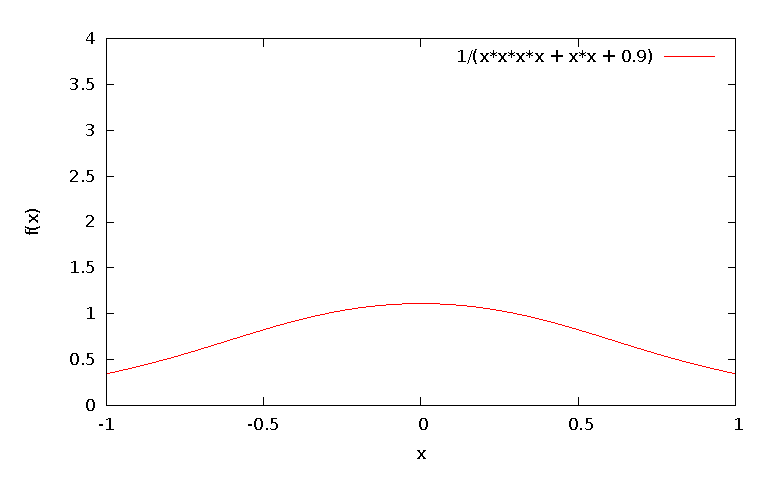
\includegraphics[width=0.8\textwidth]{wykresy/1.eps}
	    \caption{$f(x) = \frac{1}{x^4 + x^2 + 0.9}$}
	\end{figure}
	Metoda Romberga dla tej całki spełniła warunki końcowe już po wyliczeniu kolumny
	numer 7 oraz zwróciła $1.5822329637296089$.
	Tak prezentuje się tablica błędów względnych.

	\begin{table}[h]
	\centering
	\begin{tabular}[c]{|c|c|c|c|c|c|c|}
	\hline
	Lp. & 0 & 1 & 2 & \ldots & 8 & 9 \\
	\hline
	0 & $0.564125392$ &  &  &  &  & \\
	1 & $0.079820272$ & $0.081614767$ &  &  & & \\
	2 & $0.018658028$ & $0.001729386$ & $0.00359630$ & & & \\
	3 & $0.004692614$ & $3.74772453e-5$ & $0.00015526$	& \dots &  &  \\
	\dots & \dots & \dots & \dots & \dots & & \\
	8 & $4.5868371e-6$ & $1.3418809e-11$ & $4.518826e-14$ & \dots & $4.2100868e-16$ &  \\
	9 & $1.1467099e-6$ & $8.38228e-13$ & $4.210086e-16$ & \dots & $2.8067245e-16$ & $2.8067245e-16$ \\
	\hline
	\end{tabular}
	\caption{Tablica błędów względnych metody Romberga dla pierwszej całki.}
	\end{table}

	\item $\int_a^b f(x) dx = \int_0^1 \frac{1}{1 + x^4} dx \approx 0.866972987339911$ \\ \\
	\begin{figure}[H]
		\centering
		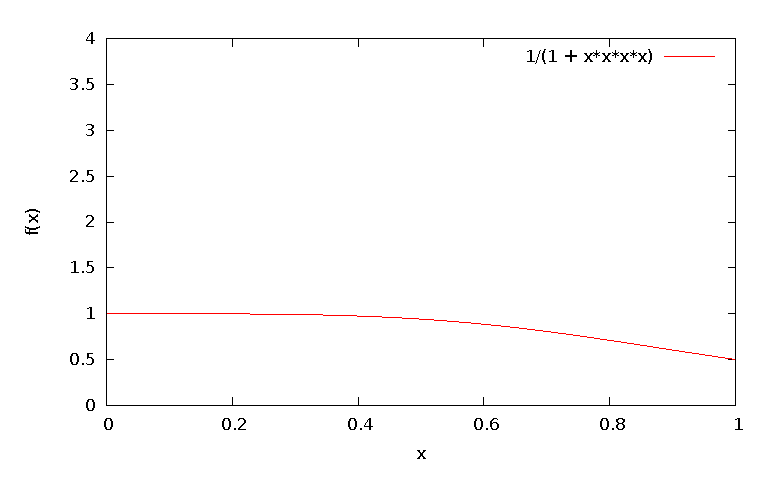
\includegraphics[width=0.8\textwidth]{wykresy/2.eps}
		\caption{$f(x) = \frac{1}{1 + x^4}$}
	\end{figure}
	Dla tej całki, metoda Romberga kończy działanie po obliczeniu kolumny nr 6.
	Otrzymano przybliżenie całki $\int_0^1 \frac{1}{1 + x^4} dx \approx 0.8669729873400975$.

	\begin{table}[h]
	\centering
	\begin{tabular}[c]{|c|c|c|c|c|c|c|}
	\hline
	Lp. & 0 & 1 & 2 & \ldots & 8 & 9 \\
	\hline
	0 & 0.1349211440	& & & & & \\
 	1 & 0.0246659957 & 0.01208572032	& & & & \\
 	2 & 0.0060447709 & 0.00016230402 & 0.0006325903 & & & \\
 	3 & 0.0015042187 & 9.298617849e-6 & 9.017423310e-7	& \dots & & \\
	\dots & \dots & \dots & \dots & \dots & & \\
	8 & 1.466675102e-6 & 8.951852211e-12 & 0.0 & \dots & 0.0 &  \\
	9 & 3.666683557e-7 & 5.599949891e-13 & 5.12229580e-16 & \dots & 5.12229580e-16 & 5.1222958e-16 \\
	\hline
	\end{tabular}
	\caption{Tablica błędów względnych metody Romberga dla drugiej całki.}
	\end{table}

	\item $\int_a^b f(x) dx = \int_0^1 \frac{2}{2 + \sin(10 \pi x)} dx \approx 1.1547005383792308$ \\ \\
	\begin{figure}[H]
		\centering
		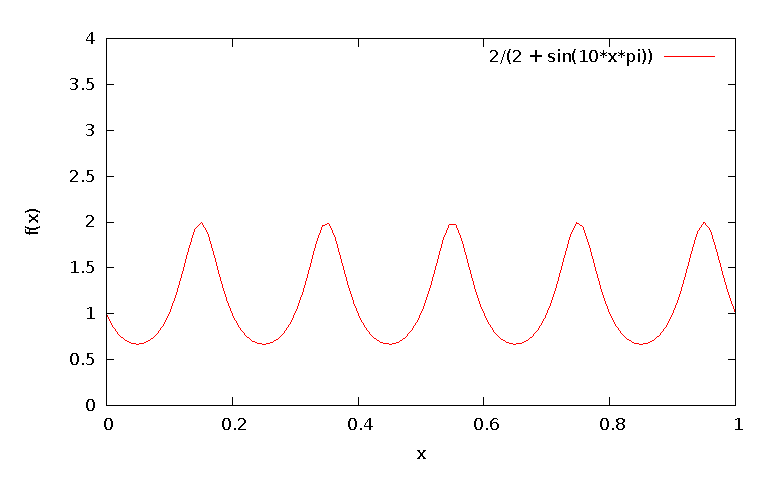
\includegraphics[width=0.8\textwidth]{wykresy/3.eps}
		\caption{$f(x) = \frac{2}{2 + \sin(10 \pi x)}$}
	\end{figure}
	W przypadku tej całki, metoda Romberga szybko kończy działanie (po wyliczeniu
	kolumny nr 1) i zwraca niepoprawny wynik $0.9999999999999999$.
	Metoda Romberga wyliczająca 10 poziomów tablicy Romberga otrzymuje już dokładny wynik $1.1547005383792495$.
	Tablica błędów wygląda następująco

	\begin{table}[h]
	\centering
	\begin{tabular}[c]{|c|c|c|c|c|c|c|}
	\hline
	Lp. & 0 & 1 & 2 & \ldots & 8 & 9 \\
	\hline
	0 & 0.1339745962 & & & & &\\
	1 & 0.1339745962 & 0.1339745962 & & & & \\
	2 & 0.0103629710 & 0.058475493 & 0.071305499 & & & \\
	3 & 5.31448463e-5 & 0.0033834638 & 0.007507394 & \dots & & \\
	\dots & \dots & \dots & \dots & \dots & & \\
	8 & 1.78835529e-14 & 1.76912567e-14 & 1.76912567e-14 & \dots & 7.86491738e-14 & \\
	9 & 1.78835529e-14 & 1.78835529e-14 & 1.78835529e-14 & \dots & 1.78835529e-14 & 1.78835529e-14 \\
	\hline
	\end{tabular}
	\caption{Tablica błędów względnych metody Romberga dla trzeciej całki.}
	\end{table}

	\item $\int_a^b f(x) dx = \int_{-200}^{200} \cos(\frac{200}{1 + x^2}) dx  \approx 364.56214839923837$ \\ \\
	Dla tej funkcji zbyt trudno narysować wykres, ponieważ w przedziale $[-1, 1]$ cosinus ,,wariuje".
	Natomiast przy $x \to \pm \infty$ funkcja $f$ dąży do jedynki.
	Metoda Romberga dla początkowych numerów kolumn odbiega od poprawnego wyniku,
	lecz poźniej dogania dokładną wartość całki zwracając $\int_{-200}^{200} \cos(\frac{200}{1 + x^2}) dx \approx 364.5621483992415$.
	\newline
	\newline
	Aby obliczyć satysfakcjonujący wynik, metoda Romberga potrzebuje policzyć aż wiersz numer 19.
	Jeśli spojrzy się na pełną tablicę błędów, można zauważyć, że w tych samych wierszach błędy mogą się
	zwiększać. Na przykład w wierszu nr 18 metoda trapezów dała przybliżenie całki o błędzie rzędu
	$10^{-15}$. Natomiast na końcu, w kolumnie 18, mamy błąd rzędu $10^{-12}$.

	\begin{table}[h]
	\centering
	\begin{tabular}[c]{|c|c|c|c|c|c|c|}
	\hline
	Lp. & 0 & 1 & 2 & \ldots & 18 & 19 \\
	\hline
	0 & 0.0971928984 &  &  &  &  & \\
	1 & 0.1841307814 & 0.2779053413 &  &  & & \\
	2 & 0.0435717793 & 0.0032812213 & 0.022026992 & & & \\
	3 & 0.0259299849 & 0.0490972396 & 0.052151640 & \dots &  &  \\
	\dots & \dots & \dots & \dots & \dots & & \\
	18 & 5.613207756e-15 & 5.769130193e-15 & 5.92505263e-15 & \dots & 1.13355612e-12	 &  \\
	19 & 7.484277008e-15 & 8.263889196e-15 & 8.41981163e-15 & \dots & 8.26388919e-15 & 8.26388919e-15\\
	\hline
	\end{tabular}
	\caption{Tablica błędów względnych metody Romberga dla czwartej całki.}
	\end{table}


	\item $\int_a^b f(x) dx = \int_{-0.9999}^{0.9999} \frac{1}{\sqrt{1 - x^2}} dx \approx 3.113308146635046$ \\ \\
	\begin{figure}[H]
		\centering
		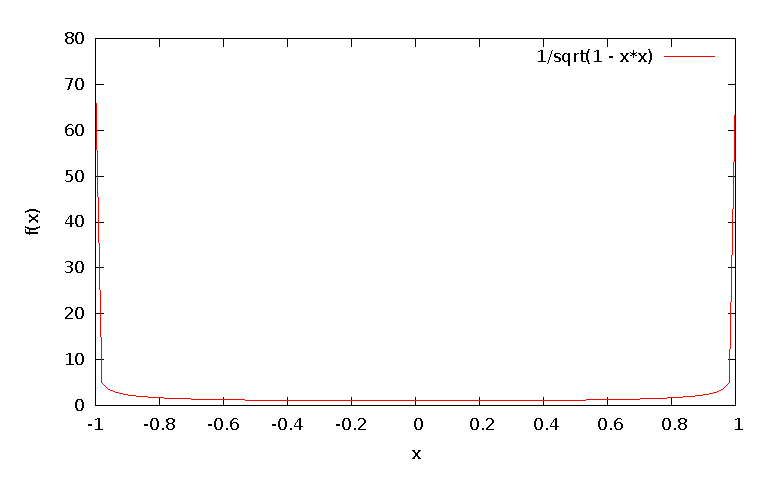
\includegraphics[width=0.8\textwidth]{wykresy/5.eps}
		\caption{$f(x) = \frac{1}{\sqrt{1 - x^2}}$}
	\end{figure}
	Metoda Romberga nie jest w stanie obliczyć całki z tej samej funkcji dla przedziału całkowania $[-1,1]$,
	ponieważ funkcja nie jest określona dla $x = \pm 1$.
	\newline
	Metoda Romberga zwraca $\int_{-0.9999}^{0.9999} \frac{1}{\sqrt{1 - x^2}} dx \approx 3.113308146650636$.
	Także i dla tej funkcji, aby osiągnąć warunki końcowe i zakończyć algorytm, potrzebne jest wyliczenie kolumny
	numer 18 w tablicy Romberga.

	\begin{table}[h]
	\centering
	\begin{tabular}[c]{|c|c|c|c|c|c|c|}
	\hline
	Lp. & 0 & 1 & 2 & \ldots & 18 & 19 \\
	\hline
	0 & 44.42137904 &  &  &  &  & \\
	1 & 22.03185914 & 14.56868584 &  &  & & \\
	2 & 10.88677194 & 7.171742881 & 6.67861335 & & & \\
	3 & 5.351986353 & 3.507057822 & 3.26274548	& \dots &  &  \\
	\dots & \dots & \dots & \dots & \dots & & \\
	18 & 2.7533692e-7 & 9.978023e-11 & 7.435939e-13 & \dots & 5.0075980e-12 &  \\
	19 & 2.7533692e-7 & 9.978023e-11 & 7.435939e-13 & \dots & 9.7139357e-14	& 9.7139357e-14	 \\
	\hline
	\end{tabular}
	\caption{Tablica błędów względnych metody Romberga dla piątej całki.}
	\end{table}

\end{enumerate}

\section{Wnioski}

Jak się okazuje, metoda Romberga faktycznie bardzo szybko przyspiesza zbieżność złożonego wzoru Trapezów.
Mogliśmy to zaobserwować w przypadku każdej funkcji.
\newline
\newline
Jednakże, istnieją funkcje, dla których metoda Romberga zwraca niepoprawny wynik. Było tak w przypadku
$\int_0^1 \frac{2}{2 + \sin(10 \pi x)} dx$. Metoda Romberga wyliczała tylko pierwsze dwie kolumy, zauważyła, że
zachodzi warunek końcowy i zakończyła działanie zwracając niepoprawny wynik. Powodem, dla którego
metoda zakończyła się, jest to, że metoda trapezów dla jednego przedziału zwraca wynik równy 1
\begin{equation*}
	f(0) = f(1) = 1 \implies h \frac{f(0) + f(1)}{2} = 1
\end{equation*}
Natomiast jeśli popatrzeć się na metodę Simpsona dzielącą przedział całkowania na 2 części, to
\begin{equation*}
	f(0) = f(1) = f(\frac{1}{2}) = 1 \implies \frac{h}{2} \frac{f(0) + 4f(\frac{1}{2} + f(1))}{3} = 1
\end{equation*}
Nic dziwnego, że metoda Romberga uznaje, że osiągnięto stabilny wynik.
\newline
\newline
Dla funkcji o ,,skomplikowanym'' wykresie jak $\frac{2}{2 + \sin(10 \pi x)}$ kwadratury dla małych $n$ będą zwracać wynik sporo
odbiegający od rzeczywistego. Mając ,,pecha'', kwadratury Newtona-Cotesa wybiorą takie węzły równoodległe,
że metoda Romberga da podobny wynik dla pierwszego wiersza danej kolumny, jak dla pierwszego wiersza kolumny poprzedniej.
\newline
\newline
To w szczególności jest prawdziwe dla funkcji okresowych. Można dobrać takie okresowe funkcje, które całkowicie zepsują nam pierwsze kolumny
tablicy Romberga. Przykładem jest chociażby trzecia badana funkcja, chociaż możnaby ją ,,usprawnić'' zwiększając jej
okresowość chociażby do $f_2(x) = \frac{2}{2 + \sin(2^{20} \pi x)}$. Można sobie tylko wyobrazić, jak bardzo
złożony wzór trapezów dla $n = 2^k$ będzie się mylił trafiając aż do $n = 2^{20}$ w punkty o wartosci 1. To samo
będzie zachodziło dla złożonego wzoru Simpsona.
\newline
\newline
Inną kwestią, na którą wartoby było zwrócić uwagę jest związek długości przedziału całkowania do liczby poziomów
tablicy Romberga, którą algorytm potrzebuje wyliczyć, by znaleźć satysfakcjonujące przybliżenie całki.
Wydaje się naturalne, że im dłuższy przedział całkownia lub im bardziej skomplikowana funkcja,
tym powinniśmy używać większej liczby węzłów w kwadraturze.
Czwarta funkcja potwierdza to, mamy przedział całkowania $[-200, 200]$, aby wyliczyć odpowiednie przybliżenie
całki, musimy wyliczyć dwadzieścia poziomów tablicy Romberga.
\newline
\newline
Natomiast piąta rozpatrywana całka pokazuje, że nie zawsze krótki przedział całkowania i stosunkowo ,,prosta'' funkcja
pozwolą nam na wyliczenie zaledwie kilku poziomów tablicy Romberga. Funkcja $\frac{1}{\sqrt{1 - x^2}}$ dla $x \to \pm 1$ dąży do nieskończoności.
Jednak nasze przedziały całkowania $[-0.9999,0.9999]$ nie znajdują się aż tak blisko $\pm 1$, ani funkcja ta
nie wydaje się specjalnie skomplikowana. Mimo to musimy policzyć aż dziewietnaście
poziomów tablicy Romberga.


\begin{thebibliography}{9}

\bibitem{Dahlquist&Bjorck}
Dahlquist, G., Bjo\"rck, A.
\emph{Numerical Methods in Scientific Computing, Volume I},
Society for Industrial and Applied Mathematics (September 4, 2008), 547-550.

\bibitem{Kincaid&Cheney}
Kincaid, D. R., Cheney, E. W.
\emph{Numerical Analysis: Mathematics of Scientific Computing}
American Mathematical Society, 2002.

\end{thebibliography}

\end{document}
